\section{Total Background Method}
The hypothesis that the $\alpha_{T}$ ratio falls exponentially in $H_T$ can be written this way:
\begin{equation}
R_{\alpha_{T}}(H_T) = A e^{-k H_T}
\end{equation}
where $A$ and $k$ are parameters whose values will be determined.  A constant ratio is equivalent to requiring $k=0$.

Let $N$ be the number of $H_T$ bins.  The bins need not have equal width.
Let $n_i$ represent the number of events observed with $\alpha_{T} > 0.55$ in each $H_T$ bin $i$.
Let $m_i$ represent the number of events observed with $\alpha_{T} \le 0.55$ in each $H_T$ bin $i$.
Then we write the likelihood for the observations in the tail this way:
\begin{equation}
L_{hadronic}=\prod_i \mathrm{Pois}(n_i |\, b_i + s_i)
\end{equation}

where $b_i$ represents the expected Standard Model background in bin $i$, 
and $s_i$ represents the expected number of signal events in bin $i$.
Systematic uncertainties are discussed in Section \ref{sec:sysUnc}.

The expected background is written thus:
\begin{equation}
b_i = \int_{x_i}^{x_{i+1}}\! \frac{\mathrm{d}N}{\mathrm{d}H_T}(x) A e^{-k x}\, \mathrm{d}x.
\end{equation}

where $\frac{\mathrm{d}N}{\mathrm{d}H_T}$ is the distribution of $H_T$ for events with $\alpha_{T} \le 0.55$,
$x_i$ is the lower edge of the bin, and $x_{i+1}$ is the upper edge of the bin ($\infty$ for the final bin).

\subsection{Delta-function $H_T$ distribution}
\label{sec:diracDeltaHt}
Assume
\begin{equation}
\frac{\mathrm{d}N}{\mathrm{d}H_T}(x) = m_{i}\delta(x-\langle H_T \rangle_i),
\end{equation}
i.e. within a bin the whole distribution occurs at the mean value of $H_T$ in that bin.
Then
\begin{equation}
b_i = \int_{x_i}^{x_{i+1}}\! m_{i}\delta(x-\langle H_T \rangle_i) Ae^{-kx}\, \mathrm{d}x = m_{i} Ae^{-k \langle H_T \rangle_i}.
\label{eq:biDirac}
\end{equation}

\subsection{Exponential $H_T$ distribution}
\label{sec:expHt}
Assume
\begin{equation}
\frac{\mathrm{d}N}{\mathrm{d}H_T}(x) = C_{i}e^{-B_{i}x}, 
\end{equation}
i.e. the distribution of $H_T$ falls exponentially in each bin, but with potentially different parameter values.
Then
\begin{equation}
b_i = \int_{x_i}^{x_{i+1}}\! C_{i}e^{-B_{i}x} Ae^{-kx}\, \mathrm{d}x = \frac{AC_i}{B_i+k}(e^{-(B_i+k)x_{i}} - e^{-(B_i+k)x_{i+1}}).
\label{eq:biExp}
\end{equation}

There are $2N$ constants to determine: $N$ $B$'s and $N$ $C$'s.
Continuity implies
\begin{equation}
C_{i}e^{-B_{i}x_{i+1}} = C_{i+1}e^{-B_{i+1}x_{i+1}},
\end{equation}
providing $N-1$ constraints.
The measurements $\{m_i\}$ provide another $N$ constraints:
\begin{equation}
m_i = \int_{x_i}^{x_{i+1}}\! \frac{\mathrm{d}N}{\mathrm{d}H_T}(x) \, \mathrm{d}x = \frac{C_i}{B_i}(e^{-B_{i}x_{i}} - e^{-B_{i}x_{i+1}}).
\end{equation}
For the final constraint, we assume that $B_{N-1} = B_N$, i.e. the final two bins can be described by the same exponential function. 
Then 
\begin{equation}
B_N = \frac{\log(1+\frac{m_{N-1}}{m_N})}{x_N - x_{N-1}}
\end{equation}
and
\begin{equation}
C_N = B_{N}m_{N}e^{B_{N}x_{N}}.
\end{equation}
When $B_{i+1}$ and $C_{i+1}$ are known, then the following equation determines $B_i$:
\begin{equation}
B_i m_i = C_{i+1} e^{-B_{i+1}x_{i+1}}(e^{B_i (x_{i+1}-x_i)}-1), 
\end{equation}
which can be solved numerically.  Then
\begin{equation}
C_i = C_{i+1} e^{-x_{i+1}(B_i-B_{i+1})}.
\end{equation}

\subsubsection{Results in the case of two signal bins}

The values of $\{B_i\}$ and $\{C_i\}$, in the ``two signal bin'' version of RA1 are given in Table \ref{tab:bsandcs}
and are validated in Figure \ref{fig:validationPlots}.
\begin{table}[hb]
  \begin{tabular}{| l | c c c c |}
    \hline
    $x_i$ (GeV) & 250 & 300 & 350 & 450 \\
    \hline
    $m_i$ & 844459 & 331948 & 225649 & 110034 \\
    $B_i$ & 0.0169 & 0.0211 & 0.0112 & 0.0112 \\
    $C_i$ & 1720095 & 5984762 & 185677 & 185677 \\
    \hline
  \end{tabular}
  \caption{The numbers $\{m_i\}$ were provided by Rob.  The others were computed as discussed in Section \ref{sec:expHt}.}
  \label{tab:bsandcs}
\end{table}

\begin{figure}[ht]
  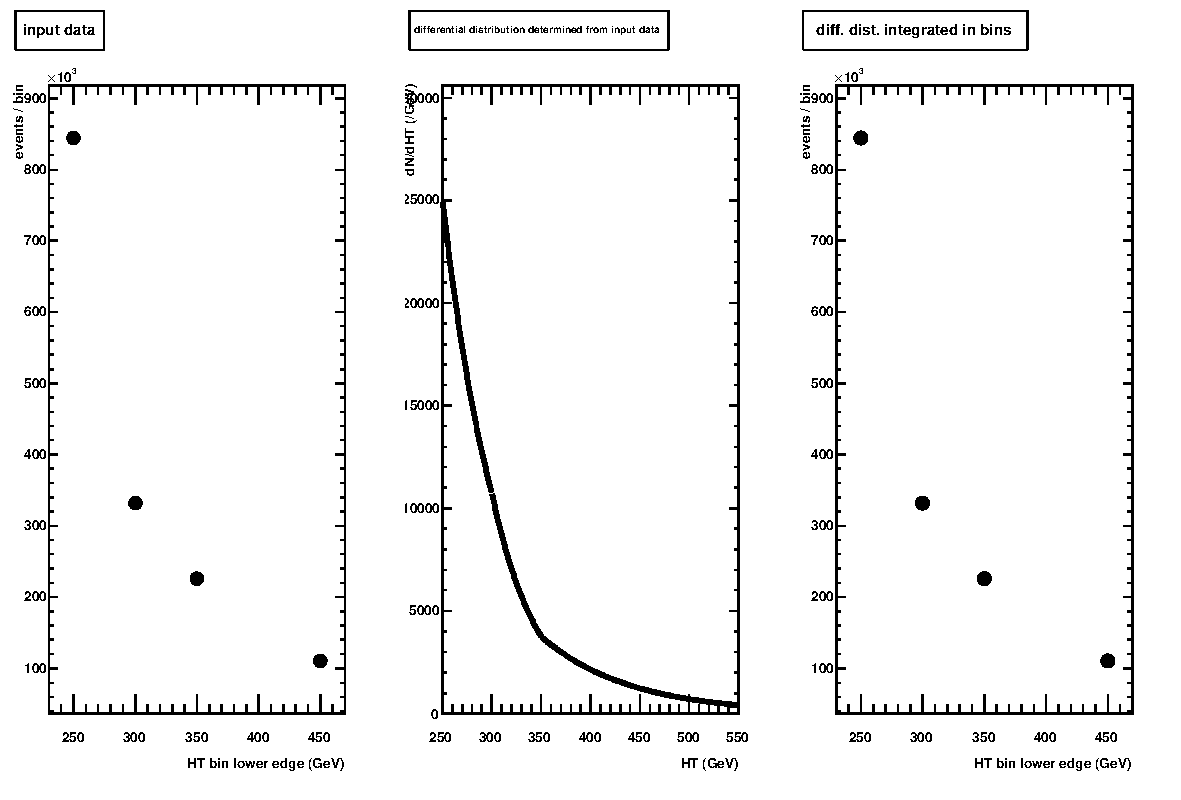
\includegraphics[width=1.2\textwidth]{totalBackgroundExpHt}
  \caption{Left: the input data.
    Middle: the $H_T$ distribution ``reconstructed'' with the exponential assumption.
    Right: the middle distribution integrated in bins.  The bin contents match the input data, i.e. the method ``closes''.}
  \label{fig:validationPlots}
\end{figure}

\subsection{Systematic Uncertainties}
\label{sec:sysUnc}
The systematic uncertainty on the assumption that $R_{\alpha_T}$ is exponential can be treated either as 
fully correlated among the bins:
\begin{equation}
L_{hadronic}=\prod_i \mathrm{Pois}(n_i |\, \tau_i b_i + s_i)\mathrm{Gaus}(\tau_i^{nominal} |\,\tau_i, \sigma)
\end{equation}

or as fully uncorrelated among the bins:

\begin{equation}
L_{hadronic}=\prod_i \mathrm{Pois}(n_i |\, \tau_i b_i + s_i)\mathrm{Gaus}(\tau_i^{nominal} |\,\tau_i, \sigma_i)
\end{equation}

or perhaps as somewhat correlated using an $N \times N$ correlation matrix.
